\documentclass[multi=tikzpicture,border=7pt]{standalone}
\usepackage{ctex,amsmath,bm}
\usepackage{tikz,pgfplots}
\pgfplotsset{compat=1.18}
\usetikzlibrary{arrows.meta,calc,angles,quotes,patterns,positioning,decorations.pathmorphing,3d,intersections}
\tikzset{wire/.style={brown!70!black,very thick},guide/.style={dashed,gray!60},force/.style={->,>=Stealth,thick,red!70!black},velocity/.style={->,>=Stealth,thick,blue!70!black},axis/.style={->,>=Stealth,thick},dim/.style={<->,>=Stealth,thin},body/.style={draw,thick,fill=blue!7},panel/.style={anchor=west,font=\bfseries},hidden/.style={dashed,gray!58,thick},orbit/.style={very thick,blue!70!black}}
\tikzset{charge/.style={circle,draw,fill=blue!12,minimum size=5.5mm,inner sep=0pt},resistor/.style={decorate,decoration={zigzag,segment length=4pt,amplitude=2pt},thick}}
\tikzset{vec/.style={->,>=Stealth,very thick},wall/.style={pattern=north east lines,pattern color=gray},nodept/.style={circle,fill=white,draw,inner sep=1.5pt}}
\begin{document}
% 1 question-01
\begin{tikzpicture}[scale=.95]
  \shade[ball color=blue!8,opacity=.45] (-3.8,0) circle(2.55);
  \draw[very thick,blue!50!black] (-3.8,0) circle(2.55);
  \foreach \a in {0,30,...,330}{\draw[blue!30] (-3.8,0)--++(\a:2.35);}
  \draw[vec] (-.75,0)--(.8,0) node[midway,above]{引力收缩};
  \shade[ball color=orange!25] (3.1,0) circle(1.25);
  \draw[very thick,orange!70!black] (3.1,0) circle(1.25);
  \foreach \a in {0,45,...,315}{\draw[orange!75!black,-Latex] (3.1,0)--++(\a:1.9);}
  \draw[dim] (3.1,0)--(4.35,0) node[midway,below]{$R$};
  \node[align=center] at (-3.8,-3.05){稀疏、近似均匀的原恒星\\质量 $M$};
  \node[align=center] at (3.1,-3.05){近似均匀的恒星\\表面温度 $T$};
\end{tikzpicture}

% 2 solution-01
\begin{tikzpicture}[x=1cm,y=1cm,font=\small]

\draw[body] (0,0) circle(1.8);\draw[blue,thick] (0,0) circle(1.1);\draw[blue,thick] (0,0) circle(1.18);
\draw[dim] (0,0)--(1.1,0) node[midway,below]{$r$};\draw[->] (2.1,1.4)--(.85,.82) node[pos=0,left]{$dm=4\pi\rho r^2dr$};
\node at (0,-2.3){$dW=Gm(r)dm/r$};\draw[->,thick] (2.5,0)--(3.3,0);
\node[draw,align=left,text width=5.7cm] at (6.4,0){$W=3GM^2/(5R)$\\[4pt]辐射：$t=W/(4\pi R^2\sigma T^4)$\\[4pt]保留内能：$T_\odot=W/(Mc)$\\[4pt]同密度：$T_*/T_\odot=(M_*/M)^{2/3}$};
\end{tikzpicture}

% 3 question-02
\begin{tikzpicture}[scale=1.05]
  \coordinate (A) at (0,2.85); \coordinate (B) at (-2.45,-1.4); \coordinate (C) at (2.45,-1.4);
  \draw[very thick] (A)--(B) (A)--(C);
  \node[charge] at (A){$A$}; \node[charge] at (B){$B$}; \node[charge] at (C){$C$};
  \node[left] at ($(A)!.55!(B)$){$l$}; \node[right] at ($(A)!.55!(C)$){$l$};
  \draw[dim] (-2.45,-2.05)--(2.45,-2.05) node[midway,below]{$l$};
  \node at (0,-2.85){初态为边长 $l$ 的正三角形，三电荷均由静止释放。};
\end{tikzpicture}

% 4 solution-02
\begin{tikzpicture}[x=1cm,y=1cm,font=\small]

\draw[guide] (0,-1.7)--(0,2.2);\draw[thick] (-1.6,-.6)--(0,1.7)--(1.6,-.6);
\node[charge] at (0,1.7){$A$};\node[charge] at (-1.6,-.6){$B$};\node[charge] at (1.6,-.6){$C$};
\draw[velocity] (0,1.4)--(0,.5) node[right]{$v$};\draw[velocity] (-1.6,-.35)--(-1.6,.4) node[left]{$v/2$};\draw[velocity] (-1.8,-.6)--(-2.6,-.6) node[below]{$u$};
\draw[dim] (-1.6,-1.3)--(1.6,-1.3) node[midway,below]{$2l\sin\theta$};
\node at (0,-2.1){$y_A=2l\cos\theta/3$};\node at (0,-2.7){$y_B=y_C=-l\cos\theta/3$};
\draw[axis] (4.5,0)--(9.3,0) node[right]{$\theta$};\draw[axis] (5,0)--(5,2.7) node[above]{$v_A^2$};
\draw[orbit] plot coordinates {(5.00000,-0.00000) (5.03770,0.01516) (5.07540,0.03165) (5.11310,0.04950) (5.15080,0.06873) (5.18850,0.08939) (5.22619,0.11149) (5.26389,0.13508) (5.30159,0.16019) (5.33929,0.18685) (5.37699,0.21510) (5.41469,0.24497) (5.45239,0.27650) (5.49009,0.30971) (5.52779,0.34464) (5.56549,0.38131) (5.60319,0.41975) (5.64088,0.45996) (5.67858,0.50197) (5.71628,0.54577) (5.75398,0.59137) (5.79168,0.63875) (5.82938,0.68788) (5.86708,0.73872) (5.90478,0.79122) (5.94248,0.84530) (5.98018,0.90088) (6.01788,0.95783) (6.05558,1.01603) (6.09327,1.07531) (6.13097,1.13548) (6.16867,1.19631) (6.20637,1.25755) (6.24407,1.31892) (6.28177,1.38011) (6.31947,1.44076) (6.35717,1.50050) (6.39487,1.55893) (6.43257,1.61561) (6.47027,1.67009) (6.50796,1.72193) (6.54566,1.77064) (6.58336,1.81576) (6.62106,1.85684) (6.65876,1.89345) (6.69646,1.92518) (6.73416,1.95168) (6.77186,1.97262) (6.80956,1.98777) (6.84726,1.99693) (6.88496,2.00000) (6.92265,1.99693) (6.96035,1.98777) (6.99805,1.97262) (7.03575,1.95168) (7.07345,1.92518) (7.11115,1.89345) (7.14885,1.85684) (7.18655,1.81576) (7.22425,1.77064) (7.26195,1.72193) (7.29965,1.67009) (7.33734,1.61561) (7.37504,1.55893) (7.41274,1.50050) (7.45044,1.44076) (7.48814,1.38011) (7.52584,1.31892) (7.56354,1.25755) (7.60124,1.19631) (7.63894,1.13548) (7.67664,1.07531) (7.71434,1.01603) (7.75204,0.95783) (7.78973,0.90088) (7.82743,0.84530) (7.86513,0.79122) (7.90283,0.73872) (7.94053,0.68788) (7.97823,0.63875) (8.01593,0.59137) (8.05363,0.54577) (8.09133,0.50197) (8.12903,0.45996) (8.16673,0.41975) (8.20442,0.38131) (8.24212,0.34464) (8.27982,0.30971) (8.31752,0.27650) (8.35522,0.24497) (8.39292,0.21510) (8.43062,0.18685) (8.46832,0.16019) (8.50602,0.13508) (8.54372,0.11149) (8.58142,0.08939) (8.61911,0.06873) (8.65681,0.04950) (8.69451,0.03165) (8.73221,0.01516) (8.76991,0.00000)};
\foreach \x/\lab in {5/{\pi/6},6.88496/{\pi/2},8.76991/{5\pi/6}}{\draw[guide] (\x,0)--(\x,2.3);\node[below] at (\x,0){$\lab$};}
\node[align=center] at (6.9,-1.6){横轴为延续构型参数\\实际内角在共线后折返};
\end{tikzpicture}

% 5 question-03
\begin{tikzpicture}[scale=.9]
  \begin{scope}[xshift=-4.6cm]
    \foreach \x/\lab in {-1.0/A,1.0/B}{
      \fill[blue!10] (\x,0) ellipse (.18 and 1.65);
      \draw[very thick] (\x,0) ellipse (.18 and 1.65);
      \draw[thin] (\x,-1.65)--(\x,2.2);
      \node[below] at (\x,-1.82){$\lab$};
    }
    \draw[dim] (-1,-2.25)--(1,-2.25) node[midway,below]{$d$};
    \node at (0,2.7){插入前};
  \end{scope}
  \begin{scope}[xshift=2.3cm]
    \foreach \x/\rad/\col/\lab in {-1.1/1.55/blue/A,0/2.35/orange/C,1.1/1.55/blue/B}{
      \fill[\col!10,opacity=.9] (\x,0) ellipse (.22 and \rad);
      \draw[very thick,\col!65!black] (\x,0) ellipse (.22 and \rad);
      \node[below] at (\x,-\rad-.25){$\lab$};
    }
    \node at (0,2.95){大圆盘 $C$ 居中插入};
  \end{scope}
  \begin{scope}[xshift=8.0cm,yshift=-.15cm]
    \fill[orange!10] (0,0) ellipse (2.5 and 1.5); \draw[very thick,orange!70!black] (0,0) ellipse (2.5 and 1.5);
    \fill[blue!16] (0,0) ellipse (1.55 and .93); \draw[very thick,blue!70!black] (0,0) ellipse (1.55 and .93);
    \draw[dim] (0,0)--(2.5,0) node[midway,below]{$D/2$};
    \draw[dim] (0,0)--(1.55,0) node[midway,above]{$2.5\,\mathrm{cm}$};
    \node at (0,2.4){同轴关系的正视图};
  \end{scope}
\end{tikzpicture}

% 6 solution-03
\begin{tikzpicture}[x=1cm,y=1cm,font=\small]

\foreach \x/\lab in {0/A,1.2/C,2.4/B}{\draw[thick] (\x,-1.7)--(\x,1.7);\node[below] at (\x,-1.7){$\lab$};}
\foreach \y in {-1,-.5,0,.5,1}{\draw[force] (0,\y)--(-.5,\y);\draw[force] (0,\y)--(.5,\y);\draw[force] (2.4,\y)--(1.9,\y);\draw[force] (2.4,\y)--(2.9,\y);}
\node[align=center] at (1.2,-2.5){外面向外，缝隙面向中盘\\$F_A=\int(\sigma^2-\sigma_*^2)dS/(2\varepsilon_0)$};
\draw[axis] (4.5,0)--(9,0) node[right]{$r$};\draw[axis] (5,0)--(5,3.1) node[above]{$\sigma$};
\draw[orbit] plot coordinates {(5.00000,0.65000) (5.03392,0.65003) (5.06783,0.65012) (5.10175,0.65027) (5.13566,0.65049) (5.16958,0.65076) (5.20349,0.65110) (5.23740,0.65150) (5.27132,0.65196) (5.30523,0.65249) (5.33915,0.65307) (5.37307,0.65372) (5.40698,0.65444) (5.44090,0.65522) (5.47481,0.65607) (5.50873,0.65698) (5.54264,0.65796) (5.57655,0.65900) (5.61047,0.66012) (5.64438,0.66130) (5.67830,0.66256) (5.71221,0.66389) (5.74613,0.66529) (5.78004,0.66677) (5.81396,0.66832) (5.84788,0.66996) (5.88179,0.67167) (5.91570,0.67346) (5.94962,0.67533) (5.98353,0.67729) (6.01745,0.67934) (6.05136,0.68147) (6.08528,0.68370) (6.11919,0.68602) (6.15311,0.68844) (6.18703,0.69095) (6.22094,0.69357) (6.25486,0.69629) (6.28877,0.69912) (6.32268,0.70206) (6.35660,0.70512) (6.39051,0.70830) (6.42443,0.71160) (6.45834,0.71503) (6.49226,0.71859) (6.52618,0.72228) (6.56009,0.72613) (6.59401,0.73011) (6.62792,0.73426) (6.66183,0.73856) (6.69575,0.74303) (6.72966,0.74768) (6.76358,0.75251) (6.79749,0.75753) (6.83141,0.76276) (6.86533,0.76819) (6.89924,0.77384) (6.93316,0.77973) (6.96707,0.78586) (7.00099,0.79224) (7.03490,0.79890) (7.06881,0.80585) (7.10273,0.81310) (7.13664,0.82067) (7.17056,0.82858) (7.20448,0.83686) (7.23839,0.84552) (7.27230,0.85460) (7.30622,0.86412) (7.34014,0.87411) (7.37405,0.88461) (7.40796,0.89566) (7.44188,0.90730) (7.47579,0.91958) (7.50971,0.93255) (7.54363,0.94628) (7.57754,0.96082) (7.61145,0.97627) (7.64537,0.99270) (7.67929,1.01022) (7.71320,1.02894) (7.74711,1.04900) (7.78103,1.07056) (7.81494,1.09379) (7.84886,1.11891) (7.88277,1.14619) (7.91669,1.17592) (7.95060,1.20848) (7.98452,1.24433) (8.01844,1.28405) (8.05235,1.32835) (8.08626,1.37816) (8.12018,1.43469) (8.15409,1.49954) (8.18801,1.57493) (8.22193,1.66400) (8.25584,1.77135) (8.28975,1.90411) (8.32367,2.07400) (8.35759,2.30207) (8.39150,2.63093)};\draw[orange,thick] (5,.881)--(8.02161,.881);\draw[guide] (8.02161,0)--(8.02161,2);\draw[guide] (8.5,0)--(8.5,3.1);
\node[below] at (8.02161,0){$R$};\node[below] at (8.65,0){$R_*$};\node[above left] at (8.02161,.881){$\sigma_*$};
\node[align=center] at (6.7,-1.4){$\sigma(r)\propto(R_*^2-r^2)^{-1/2}$\\$r\to R_*^-$ 时发散};
\end{tikzpicture}

% 7 question-04
\begin{tikzpicture}[scale=.82]
  \begin{scope}[xshift=-4.6cm]
    \foreach \x in {0,1.35,...,8.1}{\fill (\x,1.0) circle(1.55pt);}
    \foreach \x in {0,2.7,5.4,8.1}{\fill (\x,-.35) circle(1.55pt);}
    \foreach \x in {0,1.35,2.7,4.05,5.4,6.75}{\draw[resistor] (\x,1)--++(1.35,0);}
    \draw[resistor] (0,-.35)--(2.7,-.35); \draw[resistor] (2.7,-.35)--(5.4,-.35); \draw[resistor] (5.4,-.35)--(8.1,-.35);
    \draw[wire] (0,-.35)--(0,1) (2.7,-.35)--(2.7,1) (5.4,-.35)--(5.4,1) (8.1,-.35)--(8.1,1);
    \draw[resistor] (1.35,2.35)--(4.05,2.35); \draw[resistor] (4.05,2.35)--(6.75,2.35);
    \draw[wire] (1.35,1)--(1.35,2.35) (4.05,1)--(4.05,2.35) (6.75,1)--(6.75,2.35);
    \draw[wire] (1.35,2.35)--(.55,2.35); \fill (.55,2.35) circle(2pt) node[left]{$A$};
    \draw[wire] (6.75,2.35)--(7.55,2.35); \fill (7.55,2.35) circle(2pt) node[right]{$B$};
    \node at (4.05,-1.15){所有电阻的阻值均为 $R$};
  \end{scope}
  \begin{scope}[xshift=-1.3cm,yshift=-4.7cm]
    \draw[wire] (0,0)--(0,2.2); \draw (0,1.1) circle(.35); \node[left] at (-.4,1.1){$V_{\rm in}$};
    \draw[resistor] (0,2.2)--(2.2,2.2) node[midway,above=.25cm]{$R_s$};
    \draw[wire] (2.2,2.2)--(8.8,2.2); \draw[wire] (0,0)--(8.8,0);
    \draw[very thick] (3.6,2.2)--(3.6,1.35) (3.25,1.35)--(3.95,1.35) (3.25,.85)--(3.95,.85) (3.6,.85)--(3.6,0); \node[right] at (3.95,1.1){$C$};
    \draw[very thick,decorate,decoration={coil,segment length=5pt,amplitude=4pt}] (5.4,2.2)--(5.4,0); \node[right] at (5.6,1.1){$L$};
    \draw[resistor] (7.1,2.2)--(7.1,0) node[right=.25cm,midway]{$R_L$};
    \draw[wire] (8.8,2.2)--(9.5,2.2) (8.8,0)--(9.5,0); \fill (9.5,2.2) circle(2pt); \fill (9.5,0) circle(2pt);
    \draw[dim] (9.95,0)--(9.95,2.2) node[midway,right]{$V_{\rm out}$};
  \end{scope}
\end{tikzpicture}

% 8 solution-04
\begin{tikzpicture}[x=1cm,y=1cm,font=\small]

\node[panel] at (0,2.2){半网络（中央电势 $V/2$）};
\draw (0,0)--(0,1)--(.3,1);\draw[resistor] (.3,1)--(2.8,1) node[midway,above]{$R$};\draw (2.8,1)--(3.1,1)--(3.1,0);
\draw[resistor] (0,0)--(1.55,0) node[midway,below]{$2R/3$};\draw[resistor] (1.55,0)--(3.1,0) node[midway,below]{$R/3$};
\node[left] at (0,0){$A$};\node[right] at (3.1,0){$M$};\node at (1.5,-1.3){$R_{AM}=R/2,\quad R_{AB}=R$};
\node[align=center] at (1.5,-2.2){镜像电势互补\\只有中央两点可短接};
\draw[axis] (4.8,-.2)--(9.6,-.2) node[right]{$\omega/\omega_0$};\draw[axis] (5,-.2)--(5,2.5) node[above]{$|H|/|H|_{\max}$};
\draw[orbit,domain=.08:4,samples=180] plot ({5+\x},{2/sqrt(1+(\x-1/\x)^2)});

\draw[guide] (5,1.4142)--(9,1.4142);\draw[guide] (5.618,0)--(5.618,1.4142);\draw[guide] (6.618,0)--(6.618,1.4142);
\node[below] at (5.618,-.2){$\omega_-$};\node[below] at (6.618,-.2){$\omega_+$};\node[right] at (7,1.55){$1/\sqrt2$};
\draw[dim] (5.618,-1)--(6.618,-1) node[midway,below]{$\Delta\omega$};\node at (7.2,-2.2){示例：$a=1/2$};
\end{tikzpicture}

% 9 question-05
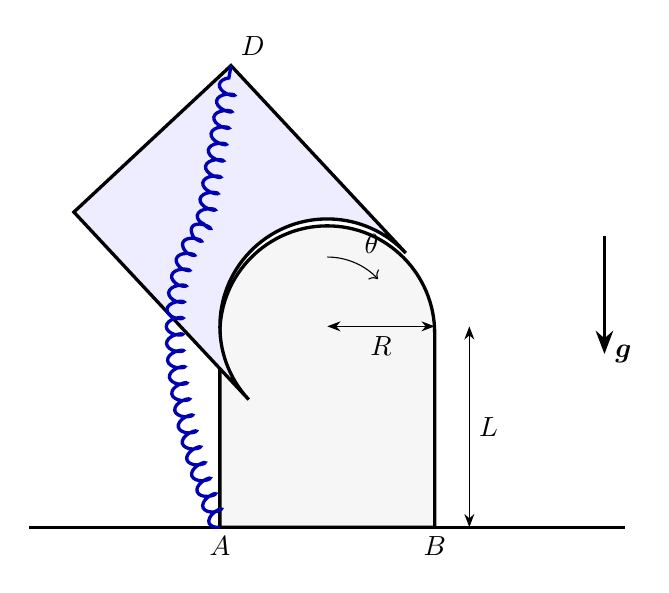
\begin{tikzpicture}[scale=.88]
  \draw[very thick] (-4.3,-2.9)--(4.3,-2.9);
  \coordinate (O) at (0,0); \fill (O) circle(2pt) node[below left]{$O$};
  \coordinate (D) at ({1.55*cos(43)-3.7*sin(43)},{1.55*sin(43)+3.7*cos(43)});
  \draw[very thick,fill=gray!7] (-1.55,-2.9)--(-1.55,-.1) arc (180:0:1.55)--(1.55,-2.9)--cycle;
  \node[below] at (-1.55,-2.9){$A$}; \node[below] at (1.55,-2.9){$B$};
  \begin{scope}[rotate=43]
    \draw[very thick,fill=blue!7] (-1.55,0)--(-1.55,3.7)--(1.55,3.7)--(1.55,0) arc (0:180:1.55)--cycle;
    \node[above right] at (1.55,3.7){$D$};
  \end{scope}
  \draw[blue!70!black,very thick,decorate,decoration={coil,aspect=.45,segment length=6pt,amplitude=3pt}]
  (-1.55,-2.9) .. controls (-2.35,-1.0) and (-2.4,.75) .. (-1.78,1.45) -- (D);
  \draw[->] (0,1.0) arc (90:43:1.0) node[midway,above right]{$\theta$};
  \draw[dim] (0,0)--(1.55,0) node[midway,below]{$R$}; \draw[dim] (2.05,-2.9)--(2.05,0) node[midway,right]{$L$};
  \draw[vec] (4.0,1.3)--(4.0,-.4) node[right]{$\bm g$};
\end{tikzpicture}

% 10 solution-05
\begin{tikzpicture}[x=1cm,y=1cm,font=\small]

\node[panel] at (0,2.8){上刚体：$\theta=0$};\draw[body] (-.9,0) rectangle (.9,2);\fill (0,0) circle(2pt) node[below]{$O$};\fill (0,1) circle(2pt) node[right]{$C$};
\draw[force] (-.9,2)--(-.9,1.2) node[left]{$kL$};\draw[force] (0,1)--(0,.3) node[right]{$mg$};\draw[force] (0,0)--(-1.4,0) node[below]{$F_{\parallel}$};\draw[force] (0,0)--(0,-.85) node[right]{$F_\perp$};
\node[align=center] at (0,-1.7){$F_{\parallel}$ 向左\\$F_\perp$ 为向下的代数分量};
\node[panel] at (4.3,2.8){下刚体：假设静止时};\draw[body] (4.5,0) rectangle (6.3,2);\draw[thick] (4,0)--(7,0);\fill (5.4,2) circle(2pt) node[above]{$O$};
\draw[force] (4.5,0)--(4.5,.8) node[left]{$kL$};\draw[force] (5.4,2)--(6.7,2) node[above]{$F_{\parallel}$};\draw[force] (5.4,2)--(5.4,2.55) node[right]{$F_\perp$};\draw[force] (5.4,1)--(5.4,.3) node[right]{$mg$};\draw[force] (6.1,0)--(4.9,0) node[midway,below]{$f$};\draw[force] (6.1,0)--(6.1,.85) node[right]{$N$};
\node[align=center] at (5.5,-1.65){$N=kL[4\beta+1-(1+\pi\alpha)^2]$\\题设下 $N<0$，静止假设不成立};
\end{tikzpicture}

% 11 question-06
\begin{tikzpicture}[scale=.95]
  \draw[very thick] (-3,-1.4)--(-3,1.4)--(3,1.4)--(3,-1.4);
  \fill[gray!25] (-1.15,-1.35) rectangle (-.85,1.35); \draw[very thick] (-1.15,-1.4)--(-1.15,1.4) (-.85,-1.4)--(-.85,1.4);
  \draw[very thick] (-1,0)--(1.45,0); \fill (1.45,0) circle(2pt);
  \fill[blue!8] (-2.95,-1.35) rectangle (-1.15,1.35);
  \node at (-2.05,0){$2.00\ \mathrm{mol}$};
  \draw[vec,blue] (-1,1.85)--(-2.4,1.85) node[midway,above]{压缩};
  \draw[vec,orange!80!black] (-1,-1.85)--(.9,-1.85) node[midway,below]{膨胀};
  \draw[dim] (-3,-2.55)--(3,-2.55) node[midway,below]{$V$ 可变};
  \node[align=center] at (6.25,0){$1\to2$：等温压缩\\$2\to3$：绝热膨胀\\$3\to4$：等温膨胀\\$4\to1$：等容升温};
\end{tikzpicture}

% 12 solution-06
\begin{tikzpicture}[x=1cm,y=1cm,font=\small]

\draw[axis] (0,0)--(4.8,0) node[right]{$V/V_0$};\draw[axis] (0,0)--(0,5) node[above]{$P$};
\draw[blue,thick] plot coordinates {(1.00000,4.40000) (1.02000,4.31373) (1.04000,4.23077) (1.06000,4.15094) (1.08000,4.07407) (1.10000,4.00000) (1.12000,3.92857) (1.14000,3.85965) (1.16000,3.79310) (1.18000,3.72881) (1.20000,3.66667) (1.22000,3.60656) (1.24000,3.54839) (1.26000,3.49206) (1.28000,3.43750) (1.30000,3.38462) (1.32000,3.33333) (1.34000,3.28358) (1.36000,3.23529) (1.38000,3.18841) (1.40000,3.14286) (1.42000,3.09859) (1.44000,3.05556) (1.46000,3.01370) (1.48000,2.97297) (1.50000,2.93333) (1.52000,2.89474) (1.54000,2.85714) (1.56000,2.82051) (1.58000,2.78481) (1.60000,2.75000) (1.62000,2.71605) (1.64000,2.68293) (1.66000,2.65060) (1.68000,2.61905) (1.70000,2.58824) (1.72000,2.55814) (1.74000,2.52874) (1.76000,2.50000) (1.78000,2.47191) (1.80000,2.44444) (1.82000,2.41758) (1.84000,2.39130) (1.86000,2.36559) (1.88000,2.34043) (1.90000,2.31579) (1.92000,2.29167) (1.94000,2.26804) (1.96000,2.24490) (1.98000,2.22222) (2.00000,2.20000) (2.02000,2.17822) (2.04000,2.15686) (2.06000,2.13592) (2.08000,2.11538) (2.10000,2.09524) (2.12000,2.07547) (2.14000,2.05607) (2.16000,2.03704) (2.18000,2.01835) (2.20000,2.00000) (2.22000,1.98198) (2.24000,1.96429) (2.26000,1.94690) (2.28000,1.92982) (2.30000,1.91304) (2.32000,1.89655) (2.34000,1.88034) (2.36000,1.86441) (2.38000,1.84874) (2.40000,1.83333) (2.42000,1.81818) (2.44000,1.80328) (2.46000,1.78862) (2.48000,1.77419) (2.50000,1.76000) (2.52000,1.74603) (2.54000,1.73228) (2.56000,1.71875) (2.58000,1.70543) (2.60000,1.69231) (2.62000,1.67939) (2.64000,1.66667) (2.66000,1.65414) (2.68000,1.64179) (2.70000,1.62963) (2.72000,1.61765) (2.74000,1.60584) (2.76000,1.59420) (2.78000,1.58273) (2.80000,1.57143) (2.82000,1.56028) (2.84000,1.54930) (2.86000,1.53846) (2.88000,1.52778) (2.90000,1.51724) (2.92000,1.50685) (2.94000,1.49660) (2.96000,1.48649) (2.98000,1.47651) (3.00000,1.46667) (3.02000,1.45695) (3.04000,1.44737) (3.06000,1.43791) (3.08000,1.42857) (3.10000,1.41935) (3.12000,1.41026) (3.14000,1.40127) (3.16000,1.39241) (3.18000,1.38365) (3.20000,1.37500) (3.22000,1.36646) (3.24000,1.35802) (3.26000,1.34969) (3.28000,1.34146) (3.30000,1.33333) (3.32000,1.32530) (3.34000,1.31737) (3.36000,1.30952) (3.38000,1.30178) (3.40000,1.29412) (3.42000,1.28655) (3.44000,1.27907) (3.46000,1.27168) (3.48000,1.26437) (3.50000,1.25714) (3.52000,1.25000) (3.54000,1.24294) (3.56000,1.23596) (3.58000,1.22905) (3.60000,1.22222) (3.62000,1.21547) (3.64000,1.20879) (3.66000,1.20219) (3.68000,1.19565) (3.70000,1.18919) (3.72000,1.18280) (3.74000,1.17647) (3.76000,1.17021) (3.78000,1.16402) (3.80000,1.15789) (3.82000,1.15183) (3.84000,1.14583) (3.86000,1.13990) (3.88000,1.13402) (3.90000,1.12821) (3.92000,1.12245) (3.94000,1.11675) (3.96000,1.11111) (3.98000,1.10553) (4.00000,1.10000)};
\draw[orange,thick] plot coordinates {(1.22297,3.31948) (1.24149,3.26998) (1.26000,3.22193) (1.27851,3.17527) (1.29703,3.12995) (1.31554,3.08590) (1.33405,3.04308) (1.35257,3.00143) (1.37108,2.96090) (1.38959,2.92145) (1.40811,2.88304) (1.42662,2.84563) (1.44513,2.80917) (1.46365,2.77364) (1.48216,2.73899) (1.50067,2.70520) (1.51919,2.67224) (1.53770,2.64006) (1.55621,2.60865) (1.57473,2.57799) (1.59324,2.54803) (1.61176,2.51876) (1.63027,2.49016) (1.64878,2.46220) (1.66730,2.43486) (1.68581,2.40812) (1.70432,2.38196) (1.72284,2.35636) (1.74135,2.33131) (1.75986,2.30678) (1.77838,2.28277) (1.79689,2.25925) (1.81540,2.23621) (1.83392,2.21364) (1.85243,2.19151) (1.87094,2.16983) (1.88946,2.14857) (1.90797,2.12772) (1.92649,2.10727) (1.94500,2.08721) (1.96351,2.06753) (1.98203,2.04822) (2.00054,2.02927) (2.01905,2.01066) (2.03757,1.99239) (2.05608,1.97445) (2.07459,1.95683) (2.09311,1.93952) (2.11162,1.92252) (2.13013,1.90581) (2.14865,1.88939) (2.16716,1.87325) (2.18567,1.85738) (2.20419,1.84178) (2.22270,1.82644) (2.24122,1.81135) (2.25973,1.79651) (2.27824,1.78191) (2.29676,1.76755) (2.31527,1.75341) (2.33378,1.73951) (2.35230,1.72581) (2.37081,1.71234) (2.38932,1.69907) (2.40784,1.68601) (2.42635,1.67314) (2.44486,1.66047) (2.46338,1.64799) (2.48189,1.63570) (2.50040,1.62359) (2.51892,1.61166) (2.53743,1.59990) (2.55595,1.58831) (2.57446,1.57689) (2.59297,1.56563) (2.61149,1.55453) (2.63000,1.54358) (2.64851,1.53279) (2.66703,1.52215) (2.68554,1.51166) (2.70405,1.50131) (2.72257,1.49110) (2.74108,1.48103) (2.75959,1.47110) (2.77811,1.46129) (2.79662,1.45162) (2.81513,1.44207) (2.83365,1.43265) (2.85216,1.42335) (2.87068,1.41417) (2.88919,1.40511) (2.90770,1.39616) (2.92622,1.38733) (2.94473,1.37861) (2.96324,1.36999) (2.98176,1.36149) (3.00027,1.35309) (3.01878,1.34479) (3.03730,1.33659) (3.05581,1.32849) (3.07432,1.32049) (3.09284,1.31259) (3.11135,1.30478) (3.12986,1.29706) (3.14838,1.28943) (3.16689,1.28190) (3.18540,1.27445) (3.20392,1.26708) (3.22243,1.25980) (3.24095,1.25261) (3.25946,1.24549) (3.27797,1.23846) (3.29649,1.23150) (3.31500,1.22462) (3.33351,1.21782) (3.35203,1.21110) (3.37054,1.20444) (3.38905,1.19786) (3.40757,1.19136) (3.42608,1.18492) (3.44459,1.17855) (3.46311,1.17225) (3.48162,1.16602) (3.50013,1.15985) (3.51865,1.15375) (3.53716,1.14771) (3.55568,1.14173) (3.57419,1.13582) (3.59270,1.12996) (3.61122,1.12417) (3.62973,1.11844) (3.64824,1.11276) (3.66676,1.10714) (3.68527,1.10158) (3.70378,1.09608) (3.72230,1.09062) (3.74081,1.08523) (3.75932,1.07988) (3.77784,1.07459) (3.79635,1.06935) (3.81486,1.06416) (3.83338,1.05902) (3.85189,1.05393) (3.87041,1.04889) (3.88892,1.04390) (3.90743,1.03895) (3.92595,1.03405) (3.94446,1.02920) (3.96297,1.02439) (3.98149,1.01963) (4.00000,1.01491)};
\draw[red,thick] plot coordinates {(1.00000,4.40000) (1.00557,4.36589) (1.01115,4.33223) (1.01672,4.29902) (1.02230,4.26623) (1.02787,4.23388) (1.03345,4.20194) (1.03902,4.17041) (1.04459,4.13929) (1.05017,4.10856) (1.05574,4.07823) (1.06132,4.04827) (1.06689,4.01869) (1.07247,3.98948) (1.07804,3.96063) (1.08361,3.93213) (1.08919,3.90399) (1.09476,3.87619) (1.10034,3.84872) (1.10591,3.82159) (1.11149,3.79479) (1.11706,3.76830) (1.12263,3.74213) (1.12821,3.71627) (1.13378,3.69072) (1.13936,3.66546) (1.14493,3.64050) (1.15051,3.61583) (1.15608,3.59145) (1.16165,3.56734) (1.16723,3.54352) (1.17280,3.51996) (1.17838,3.49667) (1.18395,3.47364) (1.18953,3.45088) (1.19510,3.42836) (1.20067,3.40610) (1.20625,3.38408) (1.21182,3.36231) (1.21740,3.34078) (1.22297,3.31948)};
\draw[->,blue,thick] (2.6,1.6923)--(2.4,1.8333);\draw[->,orange,thick] (2.5,1.6238)--(2.7,1.5035);
\draw[->,thick] (4,1.0149)--(4,1.1);\draw[->,red,thick] (1.09,3.9)--(1.16,3.7);
\foreach \x/\y/\lab/\pos in {4/1.1/1/right,1/4.4/2/above,1.222/{3.32}/3/right,4/1.0149/4/below}{\fill (\x,\y) circle(2pt) node[\pos]{$\lab$};}
\draw[guide] (1,0)--(1,4.4);\draw[guide] (1.222,0)--(1.222,3.32);\node[below] at (1,0){$1/4$};\node[below right] at (1.222,-.35){$15.0\ \mathrm L/V_0$};\node[below] at (4,0){$1$};
\node[align=left] at (7.3,3){$1\to2$：高温等温压缩\\$2\to3$：绝热膨胀\\$3\to4$：低温等温膨胀\\$4\to1$：等容升温};
\node[align=left] at (7.3,1){按实际状态作图\\$T_3/T_0=0.92264$\\两条等温线距离很近};
\end{tikzpicture}

% 13 question-07
\begin{tikzpicture}[scale=.9]
  \coordinate (P1) at (-4.2,-2.35); \coordinate (P2) at (3.55,-1.25);
  \coordinate (P3) at (3.55,2.55); \coordinate (P4) at (-4.2,1.45);
  \fill[gray!10] (P1)--(P2)--(P3)--(P4)--cycle;
  \draw[very thick] (P1)--(P2)--(P3)--(P4)--cycle;
  \foreach \t in {.1,.2,...,.9}{
    \draw[gray!35] ($(P1)!\t!(P2)$)--($(P4)!\t!(P3)$);
  }
  \foreach \t in {.2,.4,.6,.8}{
    \draw[gray!35] ($(P1)!\t!(P4)$)--($(P2)!\t!(P3)$);
  }
  \coordinate (Q1) at (-3.35,.45); \coordinate (Q2) at (2.65,1.30);
  \coordinate (S1) at (-3.35,-.18); \coordinate (S2) at (2.65,.67);
  \draw[dashed,gray!70] (S1)--(S2);
  \draw[dashed] (Q1)--(S1) (Q2)--(S2);
  \draw[blue!25,very thick,line width=5pt] (Q1)--(Q2);
  \draw[blue!75!black,very thick] (Q1)--(Q2);
  \draw[dim] ($(Q1)!0.48!(Q2)$)--($(S1)!0.48!(S2)$) node[midway,right]{$d$};
  \draw[dim] ($(Q1)+(-.05,.48)$)--($(Q2)+(-.05,.48)$) node[midway,above]{$l$};
  \draw[dim] ($(Q2)+(.2,-.12)$)--($(Q2)+(.2,.12)$) node[midway,right]{$2r$};
  \node at (-.2,-2.85){接地金属刻度板};
  \node[blue!70!black] at (-.05,3.05){均匀带电细绳，总电量 $q$};
\end{tikzpicture}

% 14 solution-07
\begin{tikzpicture}[x=1cm,y=1cm,font=\small]

\draw[blue,very thick] (-2,1.5)--(2,1.5) node[right]{$+q/l$};\draw[thick] (-2.5,0)--(2.5,0);\draw[red,dashed,very thick] (-2,-1.5)--(2,-1.5) node[right]{$-q/l$（像）};
\draw[dim] (-2.8,0)--(-2.8,1.5) node[midway,left]{$d$};\draw[dim] (-2.8,0)--(-2.8,-1.5) node[midway,left]{$d$};\node[below] at (0,0){接地板};
\node[align=center] at (0,-2.5){$U_e=A_e/\ell,\quad A_e=K_eq^2\ln(2d/r)$};
\draw[blue,very thick] (5,1.5)--(8,1.5);\draw[force] (5,1.5)--(4.3,1.5) node[above]{$F_e$};\draw[force] (8,1.5)--(8.7,1.5) node[above]{$F_e$};
\node[draw,align=left,text width=5cm] at (6.5,-.35){外加负载：$T=F_{\rm el}-F_e$\\[5pt]$dT/d\ell=Y_0S/l+2A_e/\ell^3$\\[5pt]读数偏大，本征值减去正偏差};
\end{tikzpicture}

% 15 question-08
\begin{tikzpicture}[scale=.95]
  \draw[->] (-.4,0)--(8.0,0) node[right]{$t$}; \draw[->] (0,-2.7)--(0,2.9) node[above]{$x$};
  \draw[blue,very thick] plot[domain=0:7.6,samples=120] (\x,{2.0*cos(100*\x)});
  \draw[dashed] (0,2.0)--(7.6,2.0) (0,-2.0)--(7.6,-2.0);
  \draw[dim] (1.8,0)--(1.8,2.0) node[midway,right]{$x_0$};
  \node[align=center] at (4,-3.4){$x(t)=x_0\cos\omega t$，$\omega=\sqrt{k/m}$};
\end{tikzpicture}

% 16 solution-08
\begin{tikzpicture}[x=1cm,y=1cm,font=\small]

\foreach \s/\a/\shift in {0/0/0,5/1.1/.605}{\begin{scope}[xshift=\s cm]
\draw[axis] (-1.8,0)--(3.2,0) node[right]{$x$};\draw[axis] (0,-1)--(0,2.8) node[above]{$U$};
\draw[blue,thick,domain=-1.5:1.5,samples=70] plot ({\x+\a},{\x*\x-\shift});
\draw[orange,dashed] (-1.4,{.5-\shift})--({2+\a},{.5-\shift});\draw[dim] ({\a-1},{.5-\shift})--({\a+1},{.5-\shift}) node[midway,above]{$2x_0$};
\draw[guide] (\a,-.8)--(\a,2.1);\node[below] at (\a,-.8){$x_{\rm eq}=\a$（示例）};\end{scope}}
\node[align=center] at (2.6,-2){能级从势阱底部上移 $\hbar\omega/2$\\$x_0=\sqrt2\Delta x$ 为等效振幅，基态概率密度静止};
\end{tikzpicture}

\end{document}
